\documentclass[final]{article}
\usepackage{fixme}
\usepackage{graphicx}
\usepackage[utf8x]{inputenc}
\usepackage{url}
\usepackage{acronym}
\usepackage{tikz}
\usepackage{bm}
\usepackage{subcaption}
\usepackage{listings}
\usepackage[section]{placeins}
\usepackage{etoolbox}
\preto\section\acresetall
\usetikzlibrary{calc,positioning,shapes,decorations.pathreplacing}

\tikzset{
short/.style={draw,rectangle,text height=3pt,text depth=13pt,
  text width=7pt,align=center,fill=gray!30},
long/.style={short,text width=1cm},
double/.style={short,text width=2cm}
}



\begin{document}
% the long nodes \lnode{<label>}{<right of>}
\def\snode#1#2#3{%
  \node[long,right=of #1, label=center:#3] (#2) {}}

\def\dnode#1#2#3{%
  \node[double,right=of #1, label=center:#3] (#2) {}}


\begin{titlepage}
	\begin{center}
   	{\scshape\LARGE
    	Department of Information Engineering and Computer Science\\
      	(DISI)\\
      	University of Trento, Italy\\\par}
      	\vspace{1cm}
      	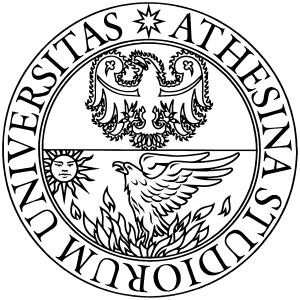
\includegraphics[scale=0.35]{logo}\\
	\vspace{1cm}
	{\scshape\Large Network Security - AY 2017/2018 \par}
	\vspace{1cm}
	{\huge\bfseries Lab Activity Report\\\par}
	\noindent\makebox[\linewidth]{\rule{\linewidth}{0.4pt}}
	{\Large\bfseries Man in the Middle attacks\par}
      	\noindent\makebox[\linewidth]{\rule{\linewidth}{0.4pt}}

        \vspace{.5cm}
        Author: \\
       	Gabriele Gemmi [198042] \\
				Lorenzo Brugnera [197054]
      	\vfill
      	\vfill
	\end{center}
\end{titlepage}

\section{Introduction}
\acrodef{MitM}{Man in the Middle}
\paragraph{What are \ac{MitM} attacks}
In a \ac{MitM} attack a malicious user secretly relays
and possibly alters the communication between two parties who believe they
are directly communicating with each other. The aim of the attacker is to
take the control of the communication and to intercept all relevant messages
passing between the two victims. \\
Once the attacker puts himself ``\textit{in the middle}'', he can do eavesdropping,
which means secretely listening to a private conversation of other parties without their consent.
This type of attack is very effective when the connection between the two
victims is not secure (HTTP).
In this way, all the traffic is exchanged in clear and the attacker can
easily manage to intercept sensitive data, like usernames, passwords, cookies and so on. \\
A \ac{MitM} attack can be performed on secure connections as well,
with the only difference that the attacker has to establish
two independent SSL sessions, one for each TCP connection.
Generally, browsers handle this kind of things,
notifying the user that the certificate is not valid.
A \ac{MitM} is well represented by the figure \ref{mitm}.
There are several ways to mount a \ac{MitM},
but one important requisite is that the attacker must be ``close''
to the victims.
\begin{figure}
\center
\includegraphics[width=.8\textwidth]{../figures/mitm_diagram}
\caption{Diagram of a \ac{MitM} attack}
\label{mitm}
\end{figure}


\subsection{Network attacks}

\begin{itemize}
  \item ARP poisoning
  \item DHCP (DHCPv6) poisoning
  \item Evil Twin
\end{itemize}

\subsection{Service attacks}
\subsubsection{ARP Poisoning}
\acrodef{ARP}{Address Resolution Protocol}
The \ac{ARP} is a communication protocol used to discover link layer addresses,
such as MAC addresses, associated with a given network layer address, which is typically IPv4.
This mapping between MAC and IP addresses is a critical function in the Internet protocol suite. \\
\ac{ARP} poisoning is a technique by which an attacker sends spoofed \ac{ARP} messages
onto a local area network with the purpose to alter the mapping between IP and MAC addresses.
It may allow an attacker to intercept data frames on a network, sniffing sensitive information or altering the traffic.
Often the attack is used as an opening for other attacks,
such as denial of service, man in the middle, or session hijacking.
The basic principle behind it is the exploitation of the the
\ac{ARP} protocol by sending spoofed messages onto the LAN.
This attack can be run from a compromised host on the LAN,
or from an attacker's machine that is connected directly to the target LAN.\\
Generally, the goal of the attack is to associate the attacker's MAC address
with the IP address of a victim, so that any traffic meant for the victim
will be sent to the attacker.
The diagram visible in figure \ref{arp_spoofing} shows the behaviour of the attack.
\begin{figure}
  \center
  \includegraphics[width=.8\textwidth]{../figures/arp_spoofing}
  \caption{ARP Spoofing attack diagram}
  \label{arp_spoofing}
\end{figure}

\paragraph{Countermeasures}
Several countermeasures can be adopted to prevent an \ac{ARP} poisoning attack:
\begin{itemize}
  \item \textbf{\ac{ARP} poisoning proof switches}. These smart switches uses Dynamic Arp Inspection (DAI) to detect illegitimate ARP responses. \cite{7345444}
  \item \textbf{Port-Based Network Access Control (802.1x)}. This protocol provides a mechanism to authenticate devices which want to establish a connection to LAN or WLAN network through a switch or a Wi-Fi access point. \cite{Qinggui_Hu}
  \item \textbf{Encrypted VPN}. These VPNs authenticate both client and server with a public key mechanism and so the attacker cannot intercept nor alter the communication.
\end{itemize}

\subsubsection{DHCP Poisoning}
\fxnote{Should we write a brief introduction on what is each of these things? SSL, HSTS?}
\acrodef{DHCP}{Dynamic Host Configuration Protocol}
\ac{DHCP} is a network management protocol used in networks to dynamically assign IP address to each device.
In this way, the user does not need to configure manually its device, that works in a plug and play fashion.\\
\ac{DHCP} poisoning is a technique which consists in setting up a rogue \ac{DHCP}  server controlled by the attacker.
Each time a client sends a \ac{DHCP} request, the rogue's response is supposed to arrive earlier than the real one.
When the legit response arrives, it is simply discarded.
The rogue server can advertise a fake gateway to the clients, in this way all the traffic going away from the local subnet will start to flow into the attacker machine.
Then, the attacker forwards the received traffic accordingly, so the clients will not notice any disruption in connectivity.
The diagram in figure \ref{dhcp_poisoning} explains how the attack works.
\begin{figure}
\center
\includegraphics[width=\textwidth]{../figures/dhcp_poisong}
\caption{DHCP poisoning attack diagram}
\label{dhcp_poisoning}
\end{figure}
\paragraph{Countermeasures}
Smart switches are one of the best solutions to avoid this kind of attack.
They are based on a mechanism which sets a port as trusted or untrusted.
As shown in the figure \ref{dhcp_snooping}, the router expects to receive DHCP responses only from the real DHCP server,
so all the responses which do not come from the legit server are discarded.

\begin{figure}
\center
\includegraphics[width=\textwidth]{../figures/dhcp_snooping}
\caption{DHCP snooping diagram}
\label{dhcp_snooping}
\end{figure}
\newpage
\subsubsection{Evil Twin}
\acrodef{SSID}{Service Set IDentifier}
The 802.11\footnote{\url{https://tools.ietf.org/html/rfc7494}} protocol allows
the creation of a wireless network with multiple Access Points (Extended Service Set).
This functionality is used in large environments where more than a single AP is needed.
In order to allow devices to perform handover, multiple APs, sharing the same \ac{SSID}, are set up. \\
An Evil Twin is a rouge AP added to an existing ESS to eavesdrop the communication.\\
The attacker sets up the rouge AP close to the victim that will receive it with a stronger signal than the legitimate one.
The diagram in figure \ref{evil_twin} explains the attack.
\begin{figure}[h]
  \center
  \includegraphics[width=\textwidth]{../figures/evil-twin}
  \caption{Evil Twin attack diagram}
  \label{evil_twin}
\end{figure}
\paragraph{Countermeasure}
Usually, a simple authentication (WPA) does not ensure the client that the AP is the legitimate one, because the attacker just need to discover the key.
Therefore, to prevent this attack, the client must verify the legitimacy of the AP. The 802.1x protocol implements this policy using Public Key Infrastructure (PKI).
\newpage
\section{Laboratory activity overview}
The following diagram shows the network topology we set up in order to mount all the attacks we wanted to explain. It is quite simple and composed by:
\begin{itemize}
  \item \textbf{Victim (Client)}. A Xubuntu machine where alumns simulate the behaviour of a victim visiting web pages on a browser.
  \item \textbf{Server}. A Linux machine running Apache HTTP Server that represents \textit{Internet}.
  \item \textbf{Attacker}. A Xubuntu machine used by alumns to mount the attacks.
  \item \textbf{Router}. An OpenWRT router used to interconnect the previous machines. It is also used as a DNS server.
\end{itemize}
\begin{figure}[h]
  \center
  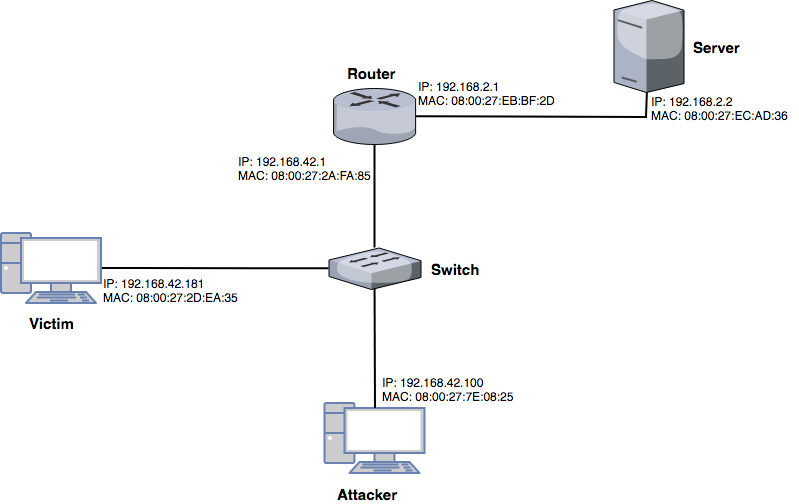
\includegraphics[width=1\textwidth]{../figures/net_topo}
  \caption{Topology of the VMs network}
\end{figure}
\newpage
\section{Exercises}
\subsection{Exercise 1 - HTTP Interception}
This preparatory exercise is used to let alumns build confidence with the machines.
Basically, in this part alumns have to capture all the traffic that flows between the victim and the router.
Since the traffic is not encrypted, sensitive information are sniffed by the attacker. \\
First of all alumns have to mount a \ac{MitM} network attack.
Theoretically any of the attacks explained before could be used.
For simplicity we chose to mount an ARP Spoofing attack using this simple command line tool available in the dsniff package\footnote{\url{https://www.monkey.org/~dugsong/dsniff/}}:
\begin{lstlisting}
arpspoof -t <victim_ip>  -r <router_ip>
\end{lstlisting}
After this, from the client virtual machine, users have to navigate to a non-secure webpage (\url{http://www.homepage.it})
and, then, using Wireshark\footnote{\url{https://www.wireshark.org/}} sniff the HTTP traffic exchanged between the victim and the server.
\subsubsection{Countermeasure}
SSL/TLS is a cryptographic protocol aimed at preserving privacy and data integrity over a computer network between two communicating computer applications.
HTTPS is the secure extension of HTTP implementing SSL/TLS.
\newpage
\subsection{Exercise 2 - SSL Stripping}
\fxnote{check the form}
Roughly speaking, SSL Strip is a technique by which every occurrence of \texttt{https://} webpage gets replaced in \texttt{http://}.
In this type of attack all the traffic from the victim’s machine is routed into the attacker's one via a transparent proxy
(sslstrip\footnote{\url{https://moxie.org/software/sslstrip/}}) that is created by the attacker himself.\\
The interesting thing is that the victim will not get any notification by the browser regarding SSL certificate errors.
The figure \ref{sslstrip} shows that the client is supposed to directly communicate with the server,
whereas all the traffic is forwarded to the attacker's machine and, then, to the server.
The diagram displayed in figure \ref{sslstrip_time} better explains all the temporal sequence of the attack.\\
\begin{figure}[h]
  \center
  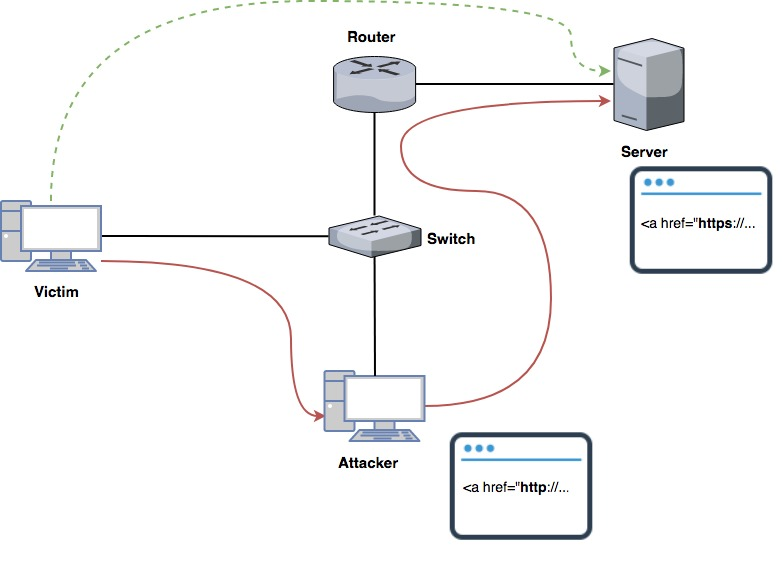
\includegraphics[width=\textwidth]{../figures/sslstrip}
  \caption{SSL Stripping attack diagram}
  \label{sslstrip}
\end{figure}
\begin{figure}[h]
  \center
  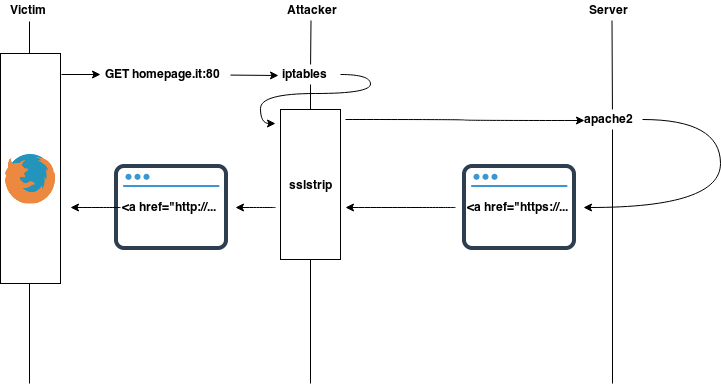
\includegraphics[width=\textwidth]{../figures/sslstrip_time}
  \caption{SSL Stripping attack diagram}
  \label{sslstrip_time}
\end{figure}
\begin{enumerate}
  \item The user agent makes a request for a non-secure webpage
  \item All the traffic reaches the attacker's virtual machine
  \item Using iptables the attacker redirects all the HTTP traffic from the port 80 to the port where sslstrip is running
  \item The HTTP traffic is forwarded to the server and the response is sent to sslstrip
  \item Sslstrip downgrades each \texttt{https://} link into an \texttt{http://} one
  \item The stripped webpage is returned to the user agent
\end{enumerate}

\noindent To properly mount this attack, the alumn have to follow this procedure:
\begin{itemize}
  \item Mount a \ac{MitM} attack
  \item Setup sslstrip to manipulate the HTTP traffic using this command line tool: \texttt{sslstrip -l <port>}
  \item Using iptables, create a specific rule to redirect the traffic from the port 80 to the port where sslstrip is running:\\
  \texttt{sudo iptables -t nat -A PREROUTING -p tcp --destination-port 80 -j REDIRECT --to-port <sslstrip\_port>}
  \item Navigate to \texttt{www.homepage.it} and click to the URL within the page
  \item Intercept the traffic using Wireshark and analyze the behaviour of sslstrip
\end{itemize}

\subsubsection{Countermeasure}
HTTP Strict Transport Security (HSTS) is a web security policy to protect against protocol downgraded attacks.
Declaring the HSTS policy, the web server forces a browser to use HTTPS.
This policy is communicated by the server to the user agent via an HTTPS response header field named \textit{Strict-Transport-Security}.
\newpage
\subsection{Exercise 3 - HSTS Bypassing}
The HSTS policy is associated with a specific domain name and changing just by one letter the domain name, the browser will
not apply the policy anymore. For instance, an ’l’ (uncapital L) could become an ’I’ (capital i).
The diagram in figure \ref{hsts_bypass} better shows the behaviour of this technique:
\begin{enumerate}
  \item The user agent makes a request for a non-secure webpage
  \item All the traffic reaches the attacker's virtual machine
  \item Using iptables the attacker redirects all the HTTP traffic from the port 80 to the port where sslstrip is running
  \item The HTTP traffic is forwarded to the server and the response is sent to sslstrip
  \item Sslstrip downgrades each \texttt{https://} link into an \texttt{http://} one, moreover it modify the domain name to something similar
  \item The stripped webpage is returned to the user agent
  \item When the user agent requests the stripped link a DNS requests is made
  \begin{figure}[h]
    \center
    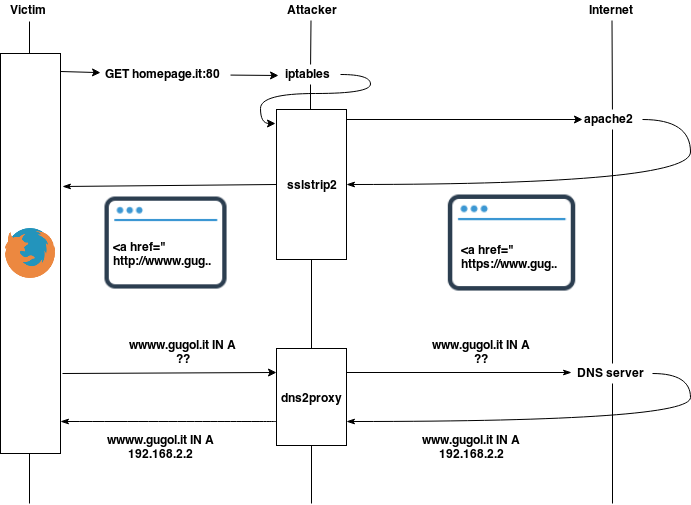
\includegraphics[width=\textwidth]{../figures/hsts_bypass_time}
    \caption{Diagram of the HSTS bypass attack}
    \label{hsts_bypass}
  \end{figure}
  \item The DNS request passes through dns2proxy and it is manipulated in order to be solved by the DNS server
  \item The legit response is received by dns2proxy, altered again and finally returned to the user
  \item The user navigates to the webpage with a slightly different domain using HTTP protocol
\end{enumerate}

\noindent To correctly mount this attack, you have to follow this procedure:
\begin{itemize}
  \item Mount a MitM attack
  \item Implement the missing code in \texttt{sslstrip/URLMonitor.py} and execute it \texttt{./sslstrip.py -l <sslstrip\_port>}
  \item Using iptables, create a specific rule to redirect the traffic from the port 80 to the port where sslstrip is running\\
  \texttt{sudo iptables -t nat -A PREROUTING -p tcp --destination-port 80 -j REDIRECT --to-port <sslstrip\_port>}
  \item Implement the missing code in \texttt{dns2proxy.py} and execute it \texttt{./dns2proxy.py}
  \item Create a specific rule to redirect all the traffic in the attacker virtual machine changing the destination ip.\\
  \texttt{sudo iptables -t nat -A PREROUTING -p udp --dport 53 -i enp0s8 -j DNAT --to <attacker\_ip>}
  \item Analyze the behaviour using Wireshark, being sure that all this trick has being working properly
\end{itemize}


\subsubsection{Countermeasures}
Unfortunately, there is no default technique to prevent this type of attack. The user must always check the correctness of the URL in the address bar.

\subsubsection{Solution of the exercise
}
\textbf{Missing code in \texttt{sslstrip/URLMonitor.py}}
\lstset{language=Python}
\begin{lstlisting}
  if host[:4] == "www.":
      fake_domain = "w" + host
  else:
      fake_domain = "web" + host

\end{lstlisting}

\noindent\textbf{Missing code in \texttt{dns2proxy.py}}
\begin{lstlisting}
  if host[:5] == 'wwww.':
      real_domain = host[1:]
  elif host[:3] == 'web':
      real_domain = host[3:]

\end{lstlisting}

\FloatBarrier
\bibliographystyle{plain}
\bibliography{main.bib}

\end{document}
